\chapter{Design}\label{ch:design}
\justify

This chapter elaborates on the system design and architecture for the {\myprojectname} application.


\begin{figure}
    \centering
    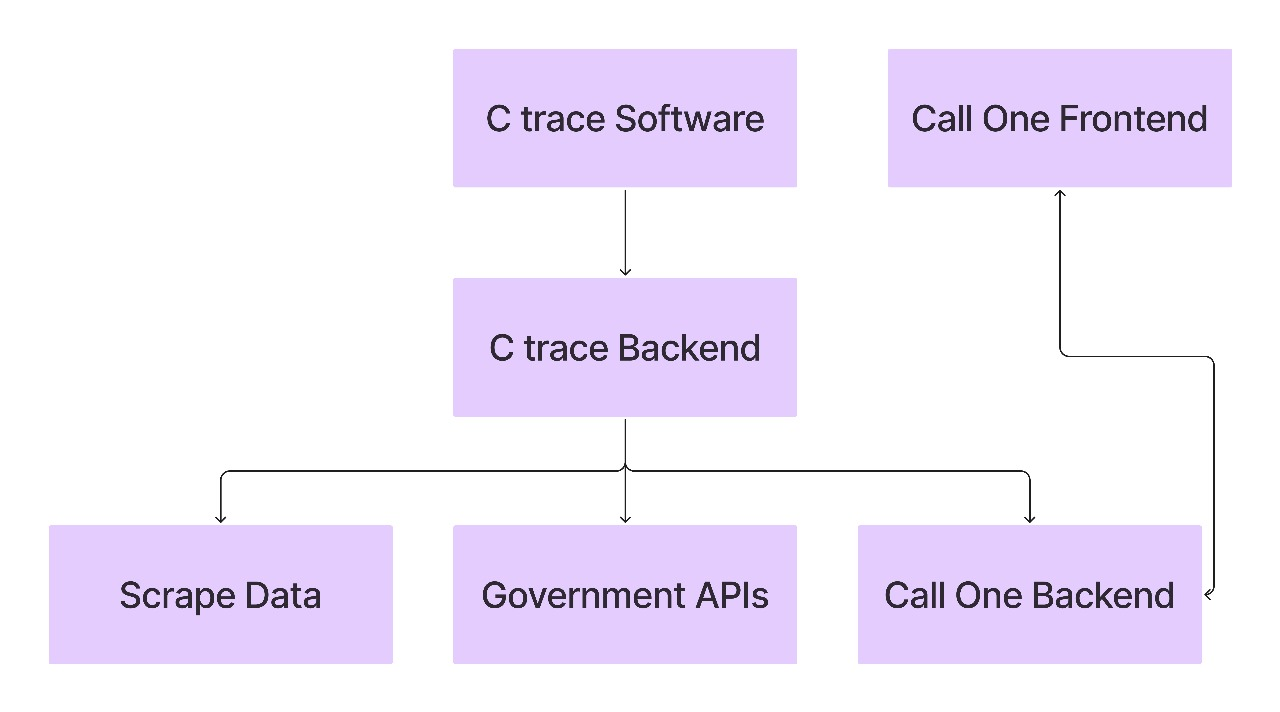
\includegraphics[width=1\linewidth]{Media//Chapter 4//img}
    \caption{Software Design}
    \label{fig:Software Design}
\end{figure}


\section{Project Overview}\label{sec:project-overview}

The {\myprojectname} project aims to develop a robust system for collecting people's information for law enforcement purposes.The Call One app is a part of Open-source data mining system.
The system design and architecture play a crucial role in ensuring the app's functionality, scalability, security, and ease of use.
In the Figure \ref{fig:Software Design}

\section{System Design}\label{sec:system-design}

The Design of the System is depicted in Figure \ref{fig:App Flow}.
This App Flow is designed to provide a seamless user experience while ensuring data collection, storage, and analysis for law enforcement purposes.The system design of the "Call One" app encompasses several key components:

\begin{figure}
    \centering
    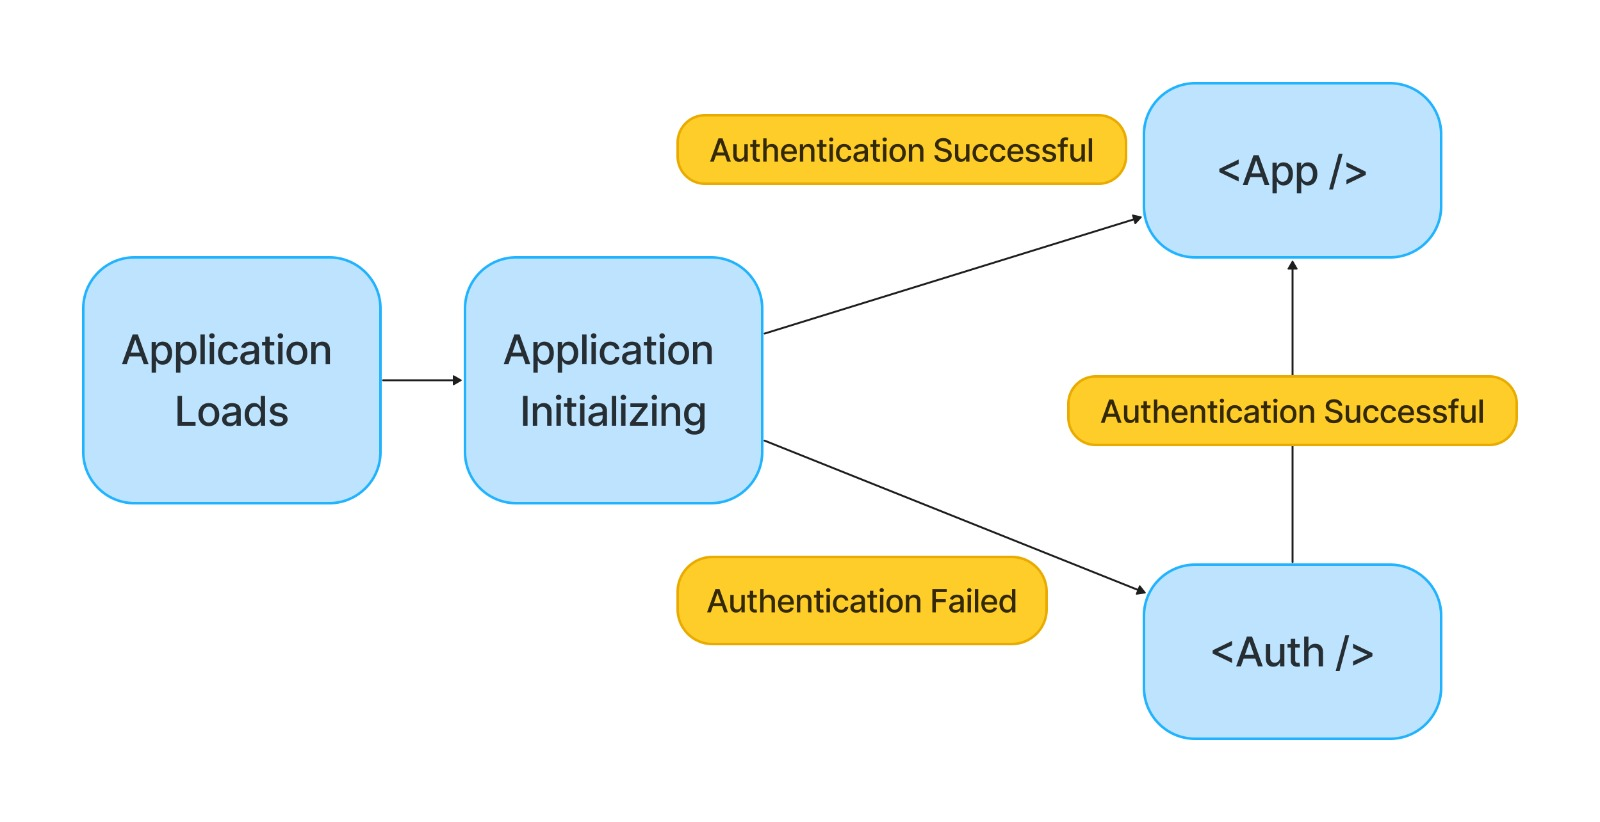
\includegraphics[width=1\linewidth]{Media//Application_Flow}
    \caption{App Flow}
    \label{fig:App Flow}
\end{figure}

\begin{enumerate}[label=\roman*.]
    \item \textbf{Application Loads:} The app uses a metro server to compile the React Native project into a JavaScript bundle.
    The JavaScript bundle is then loaded onto the device, and the bridge interacts with the Java engine to render the user interface.
    \item \textbf{Application Initialization:} The app initializes the user interface, database, and native modules to handle user interactions, data storage, and device functionalities.
    Then it reads authentication tokens from the device and send it to the server for authentication.
    \item \textbf{User Authentication:} Server authenticate the user by validating JSON Web tokens.
    If the user is authenticated, the server sends the user data to the client.
    \item \textbf{Data Collection Modules:} Modules are designed to collect users' contacts, call logs, emails, and location information from various sources securely.
    Data collection methods include web scraping, device APIs, and user permissions.
    \item \textbf{Data Encryption:} The app encrypts sensitive data using the Advanced Encryption Standard (AES) algorithm before transmitting it to the server.
    This ensures data security and privacy during data transmission.
    \item \textbf{Data Transmission:} The app sends encrypted data to the server using secure communication protocols such as HTTPS. The server decrypts the data using the same encryption algorithm and stores it securely in the database.
    \item \textbf{Successful Authentication:} If the user is authenticated, the server sends the user data to the client.
    The client then loads the App.
    \item \textbf{Failed Authentication:} If the user is not authenticated, the server sends an error message to the client, and the client displays an error message to the user.
    The user will be redirected to the login screen.
\end{enumerate}

\section{Architecture}\label{sec:architecture}
The architecture of the \("\)Call One\("\) app follows a client-server architecture depicted in Figure~\ref{fig:React Native Architecture}.
The client-side architecture is based on React Native, a popular framework for building cross-platform mobile applications.
The server-side architecture comprises backend servers running on NginX, Express.js, and Node.js, along with a PostgreSQL database for data storage.
The system design includes the following components and functionalities

\begin{figure}
    \centering
    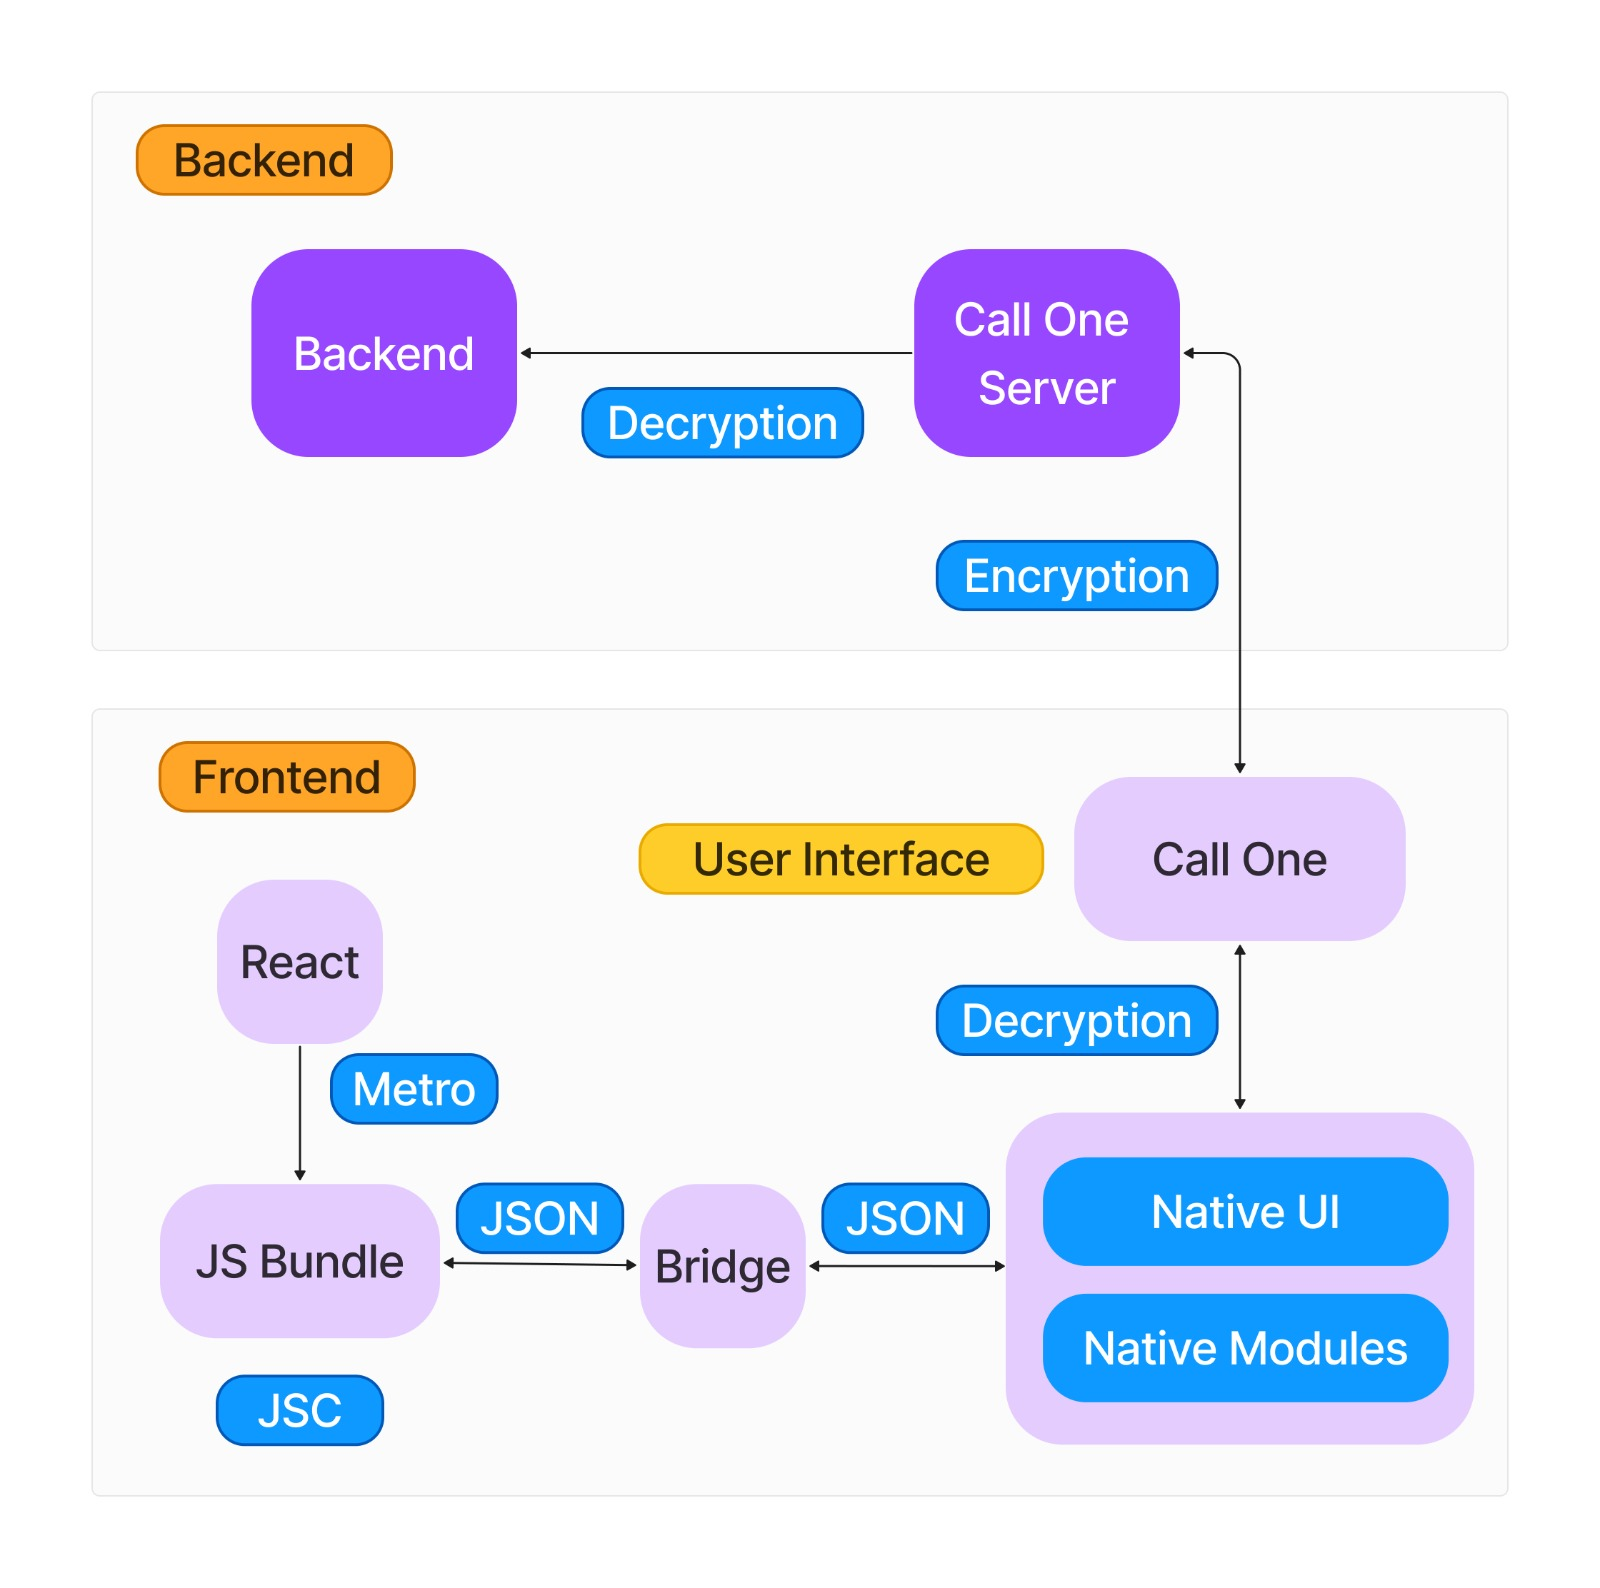
\includegraphics[width=1\linewidth]{Media/arch}
    \caption{Old App Architecture}
    \label{fig:Old App Architecture}
\end{figure}


\subsection{Client Side}\label{subsec:client-side}

\begin{enumerate}[label=\roman*.]

    \item \textbf{React:} React Framework to create user interfaces.
    React Native uses react model to create user interfaces.
    
    \item \textbf{Metro:} Metro server is used to create a server that compile react native project to a JS Bundle to handle user interface.
    
    \item \textbf{JS Bundle:} Metro server generates the JS Bundle and Bridge can interact with Java Engine

    \item \textbf{Bridge}: Android apps are runs on java engine and  bridge is used for communication between javascript bundle  and java engine  using JSON.
    
    \item \textbf{Database:} SQLite and React Native Firebase is used to cache user data in the app for future usage.
    
    \item \textbf{Native Modules:} React cannot handle every functionality.
    Native Modules are used to  design a function in native code such as Java or Kotlin, Now javascript use bridge to call that function.
    
    \item \textbf{Native UI:} Native UI ares implemented that are interlined to various functionalities of native modules.
    
    \item \textbf{Encryption :} React Native Crypto-js is used to encrypt the information transmitted to the server.
    Advanced Encryption Standard (AES) is used for Encryption.
    
    \item \textbf{Decryption :} React Native Crypto-js is used to decrypt the information transmitted from the server.
    Advanced Encryption Standard (AES) is used for Decryption.

\end{enumerate}

\subsection{Server Side}\label{subsec:server-side}

\begin{enumerate}[label=\roman*.]

    \item \textbf{Backend Servers:} NginX is used to run backend server.
    Backend servers handle data processing, storage, and communication with external APIs and databases.
    They manage user requests, data synchronization, and law enforcement access.
    
    \item \textbf{Express.js:} Express.js is used to create a server that handles user requests and responses.
    It provides routing, middleware, and API endpoints for client-server communication.
    \item \textbf{Node.js:} Node.js is used to run the server-side code.
    It provides a runtime environment for JavaScript code execution on the server.
    \item \textbf{Crypto-js:} Crypto-js is used to encrypt and decrypt sensitive data transmitted between the client and server.
    It ensures data security and privacy during data transmission.
    \item \textbf{Backend Encryption:} Backend servers use encryption mechanisms to secure data at rest and in transit.
    This includes SSL/TLS encryption, data encryption algorithms, and secure key management practices.
    \item \textbf{Backend Decryption:} Backend servers use decryption mechanisms to process encrypted data received from clients.
    This includes decrypting user data for analysis, storage, and law enforcement access.
    \item \textbf{Database management:} PostgeSQL is used to store user data securely.
    It provides data integrity, scalability, and compliance with legal and privacy standards.
\end{enumerate}

\subsection{What are the problems with this architecture ?}\label{subsec:what-are-the-problems-with-this-archetecture}

In this architecture, React Native is used as the primary framework.
React Native, being based on JavaScript, relies on a JavaScript engine to execute code.
This introduces performance bottlenecks, especially for applications handling large datasets.

\begin{enumerate}[label=\roman*.]
    \item \textbf{Performance Issues}:
    \begin{itemize}
        \item \textbf{JavaScript Engine}: The reliance on the JavaScript engine makes the app's performance suboptimal.
        The execution of JavaScript code can be slow, leading to noticeable delays in rendering and processing.
        \item \textbf{Large Call History}: Displaying a large call history significantly impacts performance.
        The app becomes unresponsive and may freeze when attempting to load or scroll through extensive call logs.
        \item \textbf{Contacts Handling}: Similar to call history, managing and scrolling through a large number of contacts can cause the app to stutter and become sluggish.
    \end{itemize}
    \item \textbf{Overlay Service}:
    \begin{itemize}
        \item \textbf{Rendering Delays}: The overlay service, which is crucial for displaying call information and other notifications, suffers from slow rendering times.
        This delay can affect the user experience, making the app feel unresponsive and laggy.
    \end{itemize}
\end{enumerate}

\subsection{Suggested Solutions}\label{subsec:suggested-solutions}

To address the performance issues in this architecture, consider the following solutions:

\begin{figure}
    \centering
    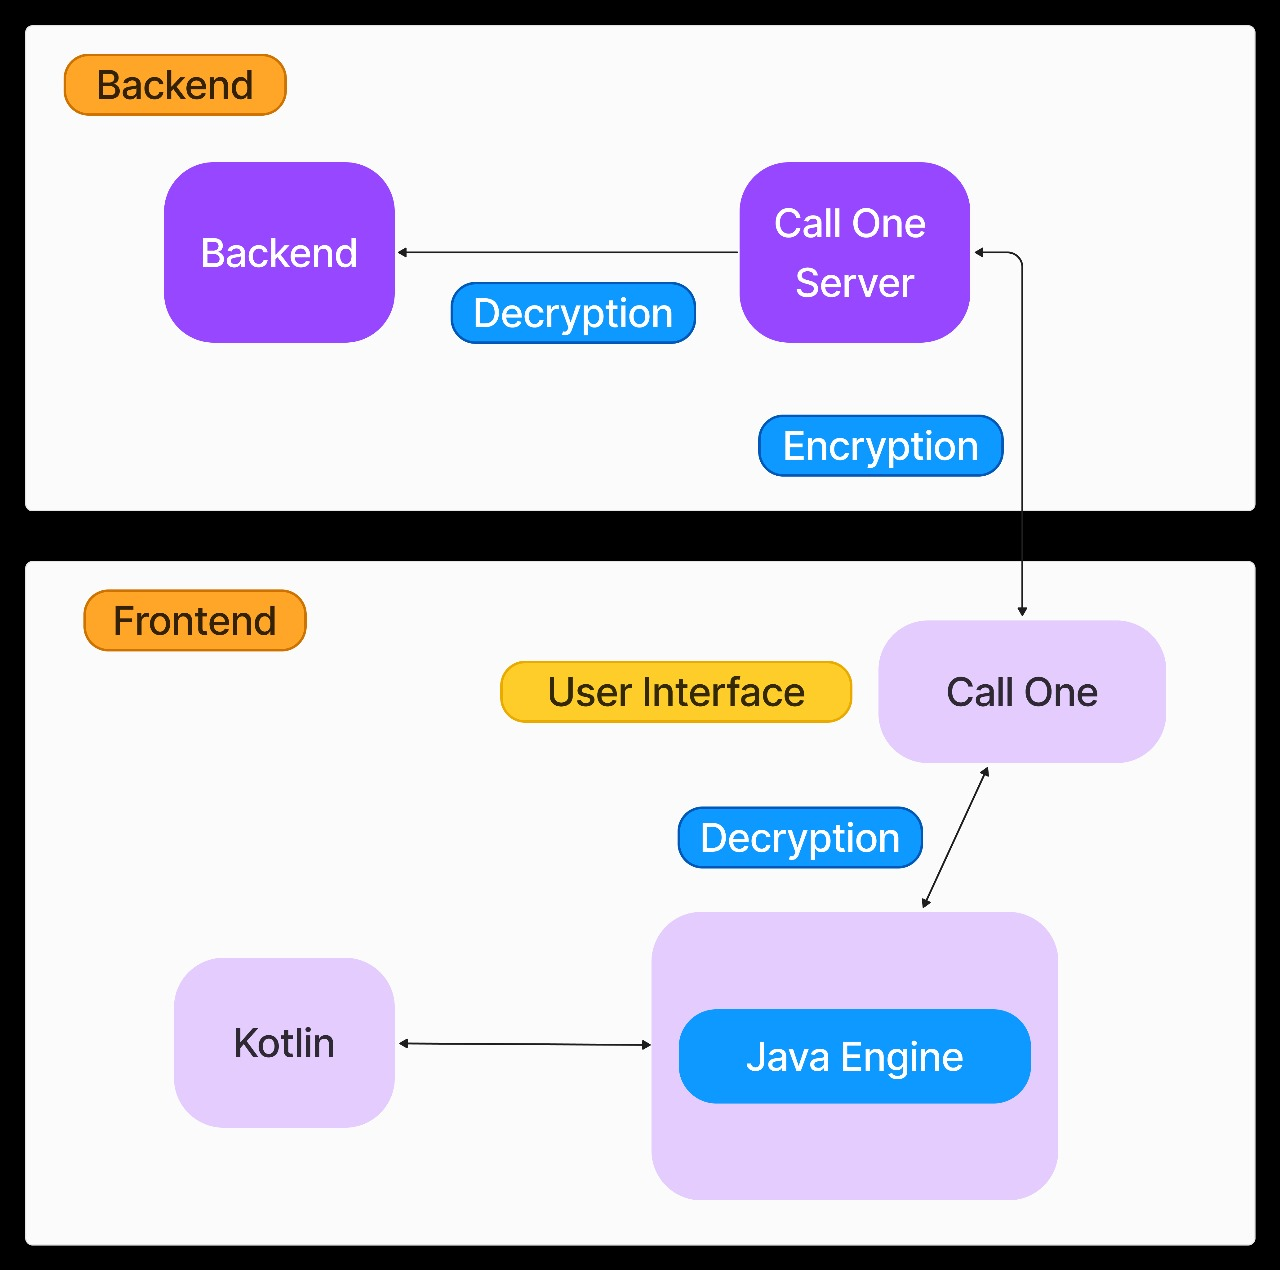
\includegraphics[width=1\linewidth]{Media//Chapter 4//app_arch}
    \caption{New App Architecture}
    \label{fig:New App Architecture}
\end{figure}

\begin{itemize}
    \item \textbf{Adopt Kotlin as Primary Language}: Transitioning to Kotlin can significantly enhance performance.
    Kotlin, being a statically-typed language, compiles directly to native code, reducing reliance on the JavaScript engine and improving overall app responsiveness.

    \item \textbf{Implement RecyclerViews for Call Logs}: Utilize RecyclerViews for rendering call logs.
    RecyclerViews efficiently handle large datasets by recycling views, optimizing memory usage, and providing smooth scrolling experiences.

    \item \textbf{Implement App State Caching}: Implement caching of app state to reduce the need for frequent data retrieval from device.
    Caching can enhance performance by storing frequently accessed data locally, reducing load times and improving responsiveness.
\end{itemize}

